INTRO

\begin{defn}
A function $f(\cdot):\mathbb{R}\rightarrow\mathbb{R}$ is said to be a \textit{squashing} function if
\begin{align}
&\lim_{x \to +\infty} f(x) = b \\
& \lim_{x \to -\infty} f(x) = a 
\end{align}
where $b,a \in \mathbb{R}$ and $b>a$
\end{defn}

Step function, ramp function and all sigmoidal functions are all examples of squashing functions.

\paragraph{Sigmoid}

\begin{align}
sigmoid(x)&= \frac{1}{1+e^{-x}}  \\ 
sigmoid'(x)&= sigmoid(x) \cdot (1-sigmoid(x))
\end{align}

As we can see from figure \ref{sigmoid_plot}, the sigmoid derivative has only one maximum in 0 where it assume value 0.25. Receding from 0, in both direction leads to regions where
the the derivative take zero value, such regions are called \textit{saturation} regions. If we happen to be in such regions, for a given neuron, we cannot learn anything since that neuron doesn't contribute
to the gradient.

\begin{figure}[h]
  \centering
    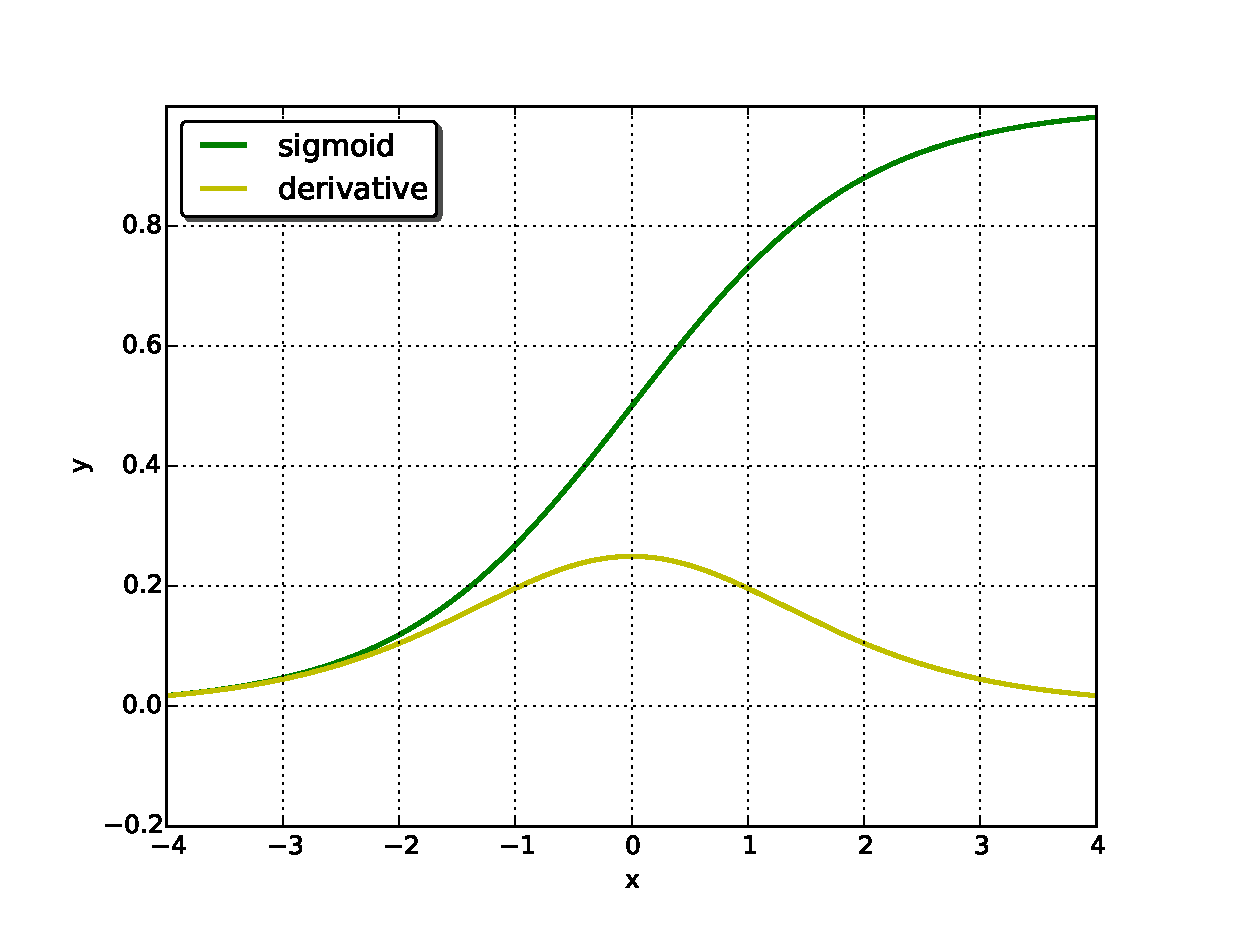
\includegraphics[width=0.9\textwidth]{sigmoid_and_deriv.eps}
  \caption{sigmoid and it's derivative}
\label{sigmoid_plot}
\end{figure}

\paragraph{Tanh}

As we can see from figure \ref{tanh_plot} tanh (and it's derivative) have a behaviour similar to the sigmoid one; Again we have two saturation region towards
infinity: that's typical of all squashing functions.

\begin{align}
 tanh(x)&=\frac{e^x-e^{-x}}{e^x+e^{-x}} \\
 tanh'(x)&= 1 - tanh^2(x)  
\end{align}

\begin{figure}[h]
  \centering
    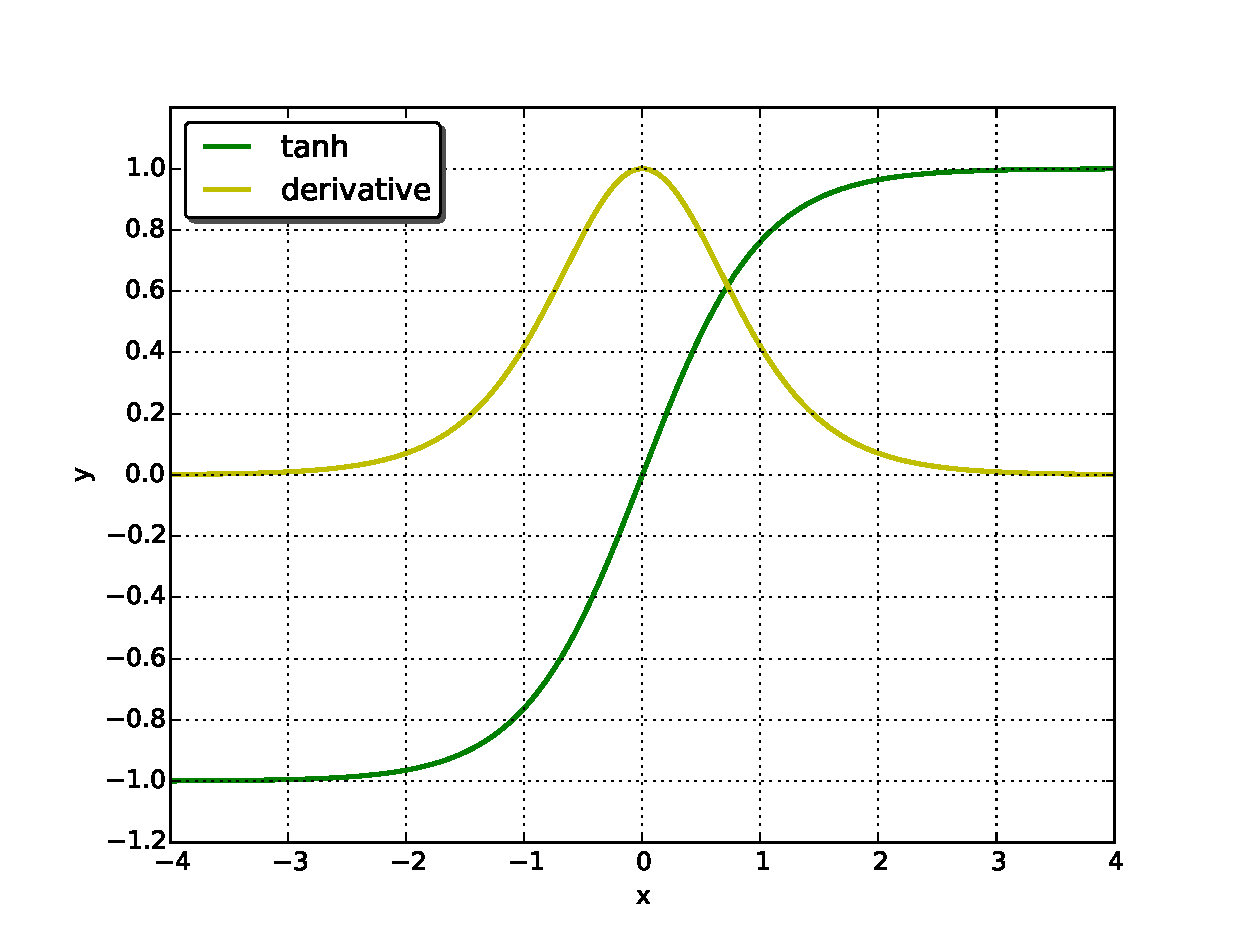
\includegraphics[width=0.9\textwidth]{tanh_and_deriv.eps}
  \caption{tanh and it's derivative}
\label{tanh_plot}
\end{figure}

\paragraph{ReLU}


\begin{align}
  ReLU(x)&=\begin{cases}
    x & \text{if $x>0$}.\\
    0 & \text{otherwise}.
  \end{cases} \\ 
   ReLU'(x)&=\begin{cases}
    1 & \text{if $x>0$}.\\
    0 & \text{otherwise}.
  \end{cases}
\end{align}


ReLU is a bit different from other activation function seen so far: the main difference is that's it's not a squashing function.
As we can see from figure \ref{relu_plot}, ReLU's derivative is the step function; it has only one \textit{saturation} region $(-\inf, 0]$ and a region in which is always takes value one, $(0,+\inf]$
This leads to the fact that we cannot learn to 'turn on' a switched off neuron ($x<0$), but we have no \textit{saturation} region toward $+\inf$.

\begin{figure}[h]
  \centering
    \includegraphics[width=0.9\textwidth]{relu_and_deriv.eps}
  \caption{ReLU and it's derivative}
\label{relu_plot}
\end{figure}
